%\documentstyle[epsf,twocolumn]{jarticle}       %LaTeX2e仕様
\documentclass[twocolumn]{jarticle}     %pLaTeX2e仕様(platex.exeの場合)
%\documentclass[twocolumn]{ujarticle}     %pLaTeX2e仕様(uplatex.exeの場合)
%%%%%%%%%%%%%%%%%%%%%%%%%%%%%%%%%%%%%%%%%%%%%%%%%%%%%%%%%%%%%%
%%
%%  基本バージョン
%%
%%%%%%%%%%%%%%%%%%%%%%%%%%%%%%%%%%%%%%%%%%%%%%%%%%%%%%%%%%%%%%%%
\setlength{\topmargin}{-45pt}
%\setlength{\oddsidemargin}{0cm} 
\setlength{\oddsidemargin}{-7.5mm}
%\setlength{\evensidemargin}{0cm} 
\setlength{\textheight}{24.1cm}
%setlength{\textheight}{25cm} 
\setlength{\textwidth}{17.4cm}
%\setlength{\textwidth}{172mm} 
\setlength{\columnsep}{11mm}

\kanjiskip=.07zw plus.5pt minus.5pt


% 【節が変わるごとに (1.1)(1.2) … (2.1)(2.2) と数式番号をつけるとき】
%\makeatletter
%\renewcommand{\theequation}{%
%\thesection.\arabic{equation}} %\@addtoreset{equation}{section}
%\makeatother

%\renewcommand{\arraystretch}{0.95} 行間の設定

%%%%%%%%%%%%%%%%%%%%%%%%%%%%%%%%%%%%%%%%%%%%%%%%%%%%%%%%
\usepackage[dvipdfmx]{graphicx}   %pLaTeX2e仕様(\documentstyle ->\documentclass)\documentclass[dvipdfmx]{graphicx}
\usepackage[dvipdfmx]{color}
\usepackage[subrefformat=parens]{subcaption}
\usepackage{colortbl}
\usepackage{multicol}
%%%%%%%%%%%%%%%%%%%%%%%%%%%%%%%%%%%%%%%%%%%%%%%%%%%%%%%%

\begin{document}

\twocolumn[
\noindent

\hspace{1em}
2021年03月05日
\hfill
\ \ 細川 岳大

\vspace{2mm}

\hrule

\begin{center}
{\Large \bf 進捗報告}
\end{center}
\hrule
\vspace{3mm}
]

% ‚ここから 文章 Start!

\section{今週やったこと}

\begin{itemize}
	\item GAの実験
\end{itemize}

\section{実験の具体案}
\subsection{探索空間の縮小}
\begin{itemize}
	\item ラベル付きデータによる予測のうち top5 のラベルに対して探索
	\item 事前学習における予測ラベルについて
	ラベル付きデータとして扱うか否かの探索
\end{itemize}
\subsection{適応度の工夫}
\begin{itemize}
	\item validation data に対しての data augementation
	\item validation loss を適応度として使用
	\item 探索データ以外に誤データを train data として組み込む
\end{itemize}

\section{実験}
\subsection{実験1:誤データの組み込み}
個体の評価時に探索データにランダムなラベルを持つ誤データを
混ぜて学習させた.また validation data にも data augmentation をした.表\ref{tb:ex1_GA},\ref{tb:ex1_config}に示す.
また,選択は2個体をエリート選択,残りをトーナメント選択(k=2)とし,交叉は一様交叉,突然変異はランダム遷移を用いた.

\subsubsection{結果}
図\ref{fig:ex1_2},\ref{fig:ex1_1}と表\ref{tb:ex1_res}に結果を示す.
\begin{figure}[h]
	\begin{center}
		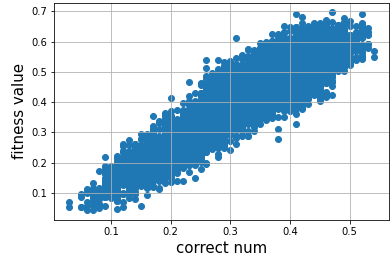
\includegraphics[height=65mm,width=90mm]{ex1_scat.png}
		\caption{実験1の散布図\label{fig:ex1_2}}
	\end{center}
\end{figure}

\begin{table}[h]
	\centering
	\caption{実験1の結果\label{tb:ex1_res}}
	\scalebox{1.0}{
		\begin{tabular}{|c|c|c|c|} \hline
			閾値&採択数&正答数&識別率\\ \hline
			なし&100&54&0.774\\ \hline
			40/50&59&40&0.762\\ \hline
			45/50&24&18&0.768\\ \hline\hline
			\multicolumn{3}{|c|}{baseline(ラベル付きデータのみ)}&0.776\\ \hline
			\multicolumn{3}{|c|}{baselineモデルによる疑似ラベル}&0.778\\
			\multicolumn{3}{|c|}{正答率(76/100)}&\\ \hline
		\end{tabular}
	}
\end{table}

図\ref{fig:ex1_2}について適応度と正答率が上がっていることが分かる.一方で,世代ごとに適応度のばらつきが激しい.これは探索データとは別で入れている誤データのラベルが世代ごとにランダムであるからだと考えられる.

また,図\ref{fig:ex1_1}について相関係数は0.9ほどであり,より相関関係が強いといえる.また,正答率ごとの適応度について最小値及び最大値がより直線的である.これにより正答率ごと平均的なの適応度もより直線的であり,前回よりも正答率が上がった理由であり,
誤データを入れたほうがより学習できるといえる.

一方表\ref{tb:ex1_res}より事前学習から得られる疑似ラベルや baseline も超えることができていないためハイパーパラメータなどの改善をする必要性がある.

改善案としてより多くの誤データを含ませることが一点,また今回誤データとして選ばれたラベルなしデータについて全て統一し,それに対するラベルは各世代ごとに統一している.これについて全世代でラベルを統一すること,また各世代ごとにラベルなしデータについても入れ替えることについても試す必要があると考えられる.

\subsection{実験2:事前学習のtop5に対する探索}
遺伝子についてこれまでとりうる値が10個あったがtop5のみに探索範囲を絞ることで5個に減らすことで探索空間の削減を狙った.また validation data にも data augmentation をした.表\ref{tb:ex2_GA},\ref{tb:ex2_config}に示す.
また,選択は2個体をエリート選択,残りをトーナメント選択(k=2)とし,交叉は一様交叉,突然変異はランダム遷移を用いた.

個体について,各遺伝子は\{0,4\}の5つのいずれかを持つ.
各遺伝子座に対応するデータの
 top5-accuracy と遺伝子\{0,4\}とがそれぞれ対応しており,
遺伝子の整数値をラベルに変換することで表現型を得る.

\subsubsection{結果}
図\ref{fig:ex2_3},\ref{fig:ex2_1}と
表\ref{tb:ex2_res}に結果を示す.

\begin{figure}[h]
	\begin{center}
		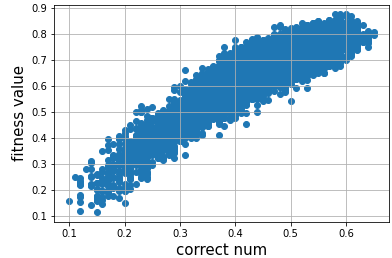
\includegraphics[height=65mm,width=90mm]{ex2_scat.png}
		\caption{実験2の散布図\label{fig:ex2_3}}
	\end{center}
\end{figure}

\begin{table}[h]
	\centering
	\caption{実験2の結果\label{tb:ex2_res}}
	\scalebox{1.0}{
		\begin{tabular}{|c|c|c|c|} \hline
			閾値&採択数&正答数&識別率\\ \hline
			なし&100&55&0.737\\ \hline
			40/50&52&37&0.759\\ \hline
			45/50&22&15&0.752\\ \hline\hline
			\multicolumn{3}{|c|}{baseline(ラベル付きデータのみ)}&0.761\\ \hline
			\multicolumn{3}{|c|}{baselineモデルによる疑似ラベル}&0.789\\
			\multicolumn{3}{|c|}{正答率(77/100)}&\\ \hline
		\end{tabular}
	}
\end{table}

結果として表\ref{tb:ex2_res}から識別率や正答率はましになったといえる.また図\ref{fig:ex2_3}について相関係数は0.9ほどであったが正答率ごとの適応度については少し曲線的であり,実験1の誤データをいれることについて検討すべきであると考えられる.

また,この実験について探索するのは10クラス識別のうち5クラスであり,探索データについて top5-accuracy は93\%であった.先ではあるが今後より難しいタスクに適応するには厳しいと考えられる.

\section{来週の課題}
\begin{itemize}
	\item 実験設定やハイパーパラメータの改良
\end{itemize}

\clearpage
\begin{figure}[t]
	\begin{center}
		\vspace*{-15mm}
		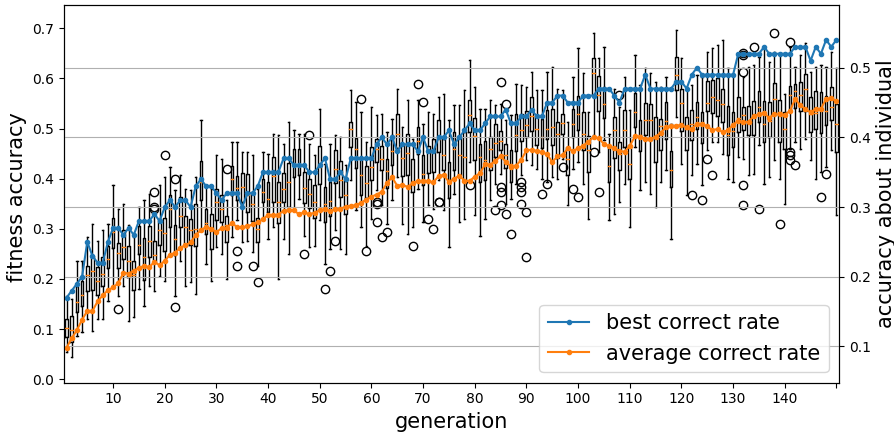
\includegraphics[height=75mm,width=180mm]{ex1_boxline.png}
		\caption{実験1 : 適応度の推移\label{fig:ex1_1}}
	\end{center}

	\begin{center}
		\vspace*{-3mm}
		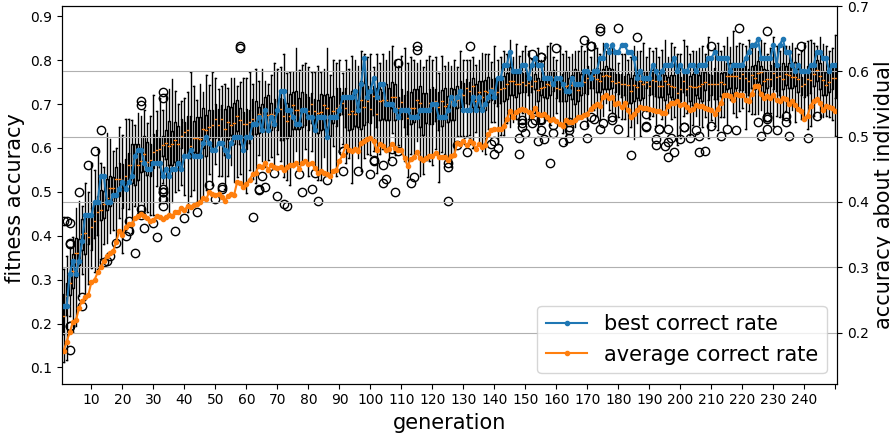
\includegraphics[height=75mm,width=180mm]{ex2_boxline.png}
		\caption{実験2 : 適応度の推移\label{fig:ex2_1}}
	\end{center}

	\begin{center}
		\vspace*{-3mm}
		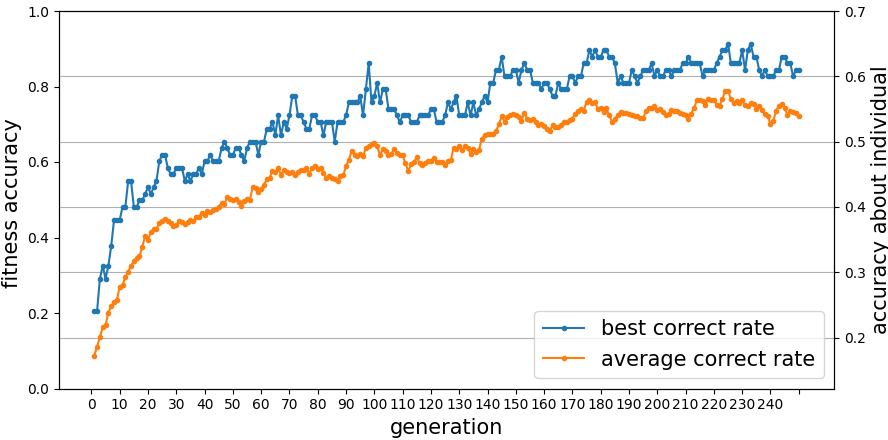
\includegraphics[height=75mm,width=180mm]{ex2_boxline2.png}
		\caption{実験2 : 適応度の推移\label{fig:ex2_2}}
	\end{center}
\end{figure}

\clearpage
\begin{table}[h]
	\centering
	\caption{実験1におけるGAの設定\label{tb:ex1_GA}}
	\scalebox{1.0}{
		\begin{tabular}{|c||c|} \hline
			ラベル付きデータ&50\\ \hline
			探索データ&100\\ \hline
			誤データ(ラベルなし)&100\\ \hline\hline
			交叉率&1.0\\ \hline
			\multicolumn{2}{|c|}{突然変異率}\\ \hline
			遺伝子ごと&0.5\\ \hline
			遺伝子座ごと&0.1\\ \hline
		\end{tabular}
	}
\end{table}

\begin{table}[h]
	\centering
	\caption{実験1におけるSimCLR の設定\label{tb:ex1_config}}
	\hspace*{-5mm}
	\scalebox{0.9}{
		\begin{tabular}{|c|c|c|} \hline
			model&Encoder&ResNet18\\ \cline{2-3}
			&Projection head&2層MLP(shape:2048to512)\\ \cline{2-3}
			&classifer&MLP(shape:2048to10)\\ \hline\hline
			\multicolumn{3}{|c|}{Encoder学習}\\ \hline
			\multicolumn{2}{|c|}{train\_data(unlabeled)}&50000\\ \hline
			batch size&\multicolumn{2}{|c|}{1024}\\ \hline
			epochs&\multicolumn{2}{c|}{500}\\ \hline
			optimizer&\multicolumn{2}{c|}
			{Adam(lr=$1.0*10^{-3}$)}\\ \hline\hline
			\multicolumn{3}{|c|}{GA 中の個体評価}\\ \hline
			\multicolumn{2}{|c|}{train\_data(labeled)}&100+100\\ \hline
			batch size&\multicolumn{2}{|c|}{32}\\ \hline
			epochs&\multicolumn{2}{c|}{10}\\ \hline
			loss&\multicolumn{2}{|c|}{Cross Entropy Loss}\\ \hline
			optimizer&\multicolumn{2}{c|}{Adam(lr=$5.0*10^{-2}$)}\\ \hline
			validation data&\multicolumn{2}{c|}{$50*3$}\\ \hline
			\multicolumn{3}{|c|}{探索された個体の評価}\\ \hline
			\multicolumn{2}{|c|}{train\_data(labeled)}&50+100\\ \hline
			batch size&\multicolumn{2}{|c|}{64}\\ \hline
			epochs&\multicolumn{2}{c|}{100}\\ \hline
			loss&\multicolumn{2}{|c|}{Cross Entropy Loss}\\ \hline
			optimizer&\multicolumn{2}{c|}{Adam(lr=$5.0*10^{-3}$)}\\ \hline
			test data&\multicolumn{2}{c|}{10000}\\ \hline
		\end{tabular}
	}
\end{table}

\begin{table}[t]
	\centering
	\caption{実験2におけるGAの設定\label{tb:ex2_GA}}
	\scalebox{1.0}{
		\begin{tabular}{|c||c|} \hline
			ラベル付きデータ&50\\ \hline
			探索データ&100\\ \hline\hline
			交叉率&1.0\\ \hline
			\multicolumn{2}{|c|}{突然変異率}\\ \hline
			遺伝子ごと&0.5\\ \hline
			遺伝子座ごと&0.1\\ \hline
		\end{tabular}
	}
\end{table}

\begin{table}[h]
	\centering
	\caption{実験2におけるSimCLR の設定\label{tb:ex2_config}}
	\scalebox{0.9}{
		\begin{tabular}{|c|c|c|} \hline
			model&Encoder&ResNet18\\ \cline{2-3}
			&Projection head&2層MLP(shape:2048to512)\\ \cline{2-3}
			&classifer&MLP(shape:2048to10)\\ \hline\hline
			\multicolumn{3}{|c|}{Encoder学習}\\ \hline
			\multicolumn{2}{|c|}{train\_data(unlabeled)}&50000\\ \hline
			batch size&\multicolumn{2}{|c|}{1024}\\ \hline
			epochs&\multicolumn{2}{c|}{500}\\ \hline
			optimizer&\multicolumn{2}{c|}
			{Adam(lr=$1.0*10^{-3}$)}\\ \hline\hline
			\multicolumn{3}{|c|}{GA 中の個体評価}\\ \hline
			\multicolumn{2}{|c|}{train\_data(labeled)}&100\\ \hline
			batch size&\multicolumn{2}{|c|}{32}\\ \hline
			epochs&\multicolumn{2}{c|}{10}\\ \hline
			loss&\multicolumn{2}{|c|}{Cross Entropy Loss}\\ \hline
			optimizer&\multicolumn{2}{c|}{Adam(lr=$5.0*10^{-2}$)}\\ \hline
			validation data&\multicolumn{2}{c|}{$50*3$}\\ \hline
			\multicolumn{3}{|c|}{探索された個体の評価}\\ \hline
			\multicolumn{2}{|c|}{train\_data(labeled)}&50+100\\ \hline
			batch size&\multicolumn{2}{|c|}{64}\\ \hline
			epochs&\multicolumn{2}{c|}{100}\\ \hline
			loss&\multicolumn{2}{|c|}{Cross Entropy Loss}\\ \hline
			optimizer&\multicolumn{2}{c|}{Adam(lr=$5.0*10^{-3}$)}\\ \hline
			test data&\multicolumn{2}{c|}{10000}\\ \hline
		\end{tabular}
	}
\end{table}

\end{document}


